\documentclass[paper=a4, fontsize=12pt]{scrreprt} % A4 paper and 11pt font size
\usepackage[T1]{fontenc} % Use 8-bit encoding that has 256 glyphs

\usepackage[english]{babel} % English language/hyphenation
\usepackage{amsmath,amsfonts,amsthm} % Math packages
\usepackage{tex_packages/register} %Register library

\usepackage{caption}
\usepackage{subcaption}
\usepackage{graphicx}
\usepackage{float}
%\usepackage[]{hyperref}  %link color

%table layout to the right
%\usepackage[labelfont=bf]{caption}
%\captionsetup[table]{labelsep=space,justification=raggedright,singlelinecheck=off}
%\captionsetup[figure]{labelsep=quad}

\usepackage{titlesec}
%\usepackage{sectsty} % Allows customizing section commands
%\renewcommand*\sectfont{\rmfamily\mdseries\itshape}
%\allsectionsfont{\normalfont} % Make all sections centered, the default font and small caps
%\allsectionsfont{ } % Make all sections centered, the default font and small caps

%\usepackage{fancyhdr} % Custom headers and footers
%\pagestyle{fancyplain} % Makes all pages in the document conform to the custom headers and footers
%\fancyhead{} % No page header - if you want one, create it in the same way as the footers below
%\fancyfoot[L]{} % Empty left footer
%\fancyfoot[C]{} % Empty center footer
%\fancyfoot[R]{\thepage} % Page numbering for right footer
%\renewcommand{\headrulewidth}{0pt} % Remove header underlines
%\renewcommand{\footrulewidth}{0pt} % Remove footer underlines
%\setlength{\headheight}{13.6pt} % Customize the height of the header

\numberwithin{equation}{section} % Number equations within sections (i.e. 1.1, 1.2, 2.1, 2.2 instead of 1, 2, 3, 4)
\numberwithin{figure}{section} % Number figures within sections (i.e. 1.1, 1.2, 2.1, 2.2 instead of 1, 2, 3, 4)
\numberwithin{table}{section} % Number tables within sections (i.e. 1.1, 1.2, 2.1, 2.2 instead of 1, 2, 3, 4)

%\setlength\parindent{0pt} % Removes all indentation from paragraphs - comment this line for an assignment with lots of text


\setlength\parskip{4pt}

%----------------------------------------------------------------------------------------
%	TITLE SECTION
%----------------------------------------------------------------------------------------

\newcommand{\horrule}[1]{\rule{\linewidth}{#1}} % Create horizontal rule command with 1 argument of height

\title{	
\normalfont \normalsize 
\horrule{0.5pt} \\[0.4cm] % Thin top horizontal rule
\huge  Traffic Injector Specifications\\ % The assignment title
\horrule{0.5pt} \\[0.4cm] % Thick bottom horizontal rule
}

\author{ Oriol Sala Sucarrats} % Your name
\date{\today} % Today's date or a custom date

\begin{document}
%\nocite{*}
\maketitle % Print the title

\newpage
\tableofcontents

\subsection{Module description}
\label{module_desc}
This unit acts as an AHB/AXI Master IP connected to the main bus on the SELENE Platform. It acts as a core with limited capabilities, only generating transactions to the bus by reading and writing to the AHB Slave RAM memory and controlled via APB registers.\\
The injector works along with the multi-core setup instantiated on the platform and other peripherals and monitoring units.\\
The module's specifications described in this section include non-implemented features, and it might be revisited for future improvements.\\
In order to generate traffic to the bus, the module performs a set of data transactions based on descriptors set at startup into a predefined memory address range.\\
The Traffic Injector is based on generic Direct Memory Access functionality fundamentals and extends its features to meet the injector objectives.\\
The internal components and respective configuration and functionalities are described in next sections.




\subsection{Operation}
\label{operation}

\subsubsection{Overview}
When the injector execution is enabled by setting the \textbf{EN} bit in the \textbf{Control APB Register}, descriptor execution starts from the first descriptor, which is pointed by the \textbf{Descriptor Pointer APB Register}. 
The injector decodes the descriptor configuration, identifies the type of transaction, and continues with the execution. On completion of each descriptor, an interrupt flag may be configured and then continues with the \textbf{next descriptor pointer} set by the current descriptor's next descriptor pointer field value. Any disabled descriptor (\textbf{EN} bit is zero in the d\textbf{escriptor control word}) will be skipped. \\
The injector should be configured such that the last descriptor has the \textbf{next.last} bit set to 1 (inside the \textbf{next descriptor pointer APB register}). After completing the last descriptor on the queue, the injector will remain \textbf{idle}.\\
All descriptors on the queue are read at startup and loaded into the internal FIFO. After that last descriptor read, the first descriptor in the FIFO will get executed and will follow the predefined order.\\
In the case of configuring the Queue Mode bit (QMode in the Control APB Register), the \textbf{next.last} bit is ignored, the last descriptor in the queue will execute the first descriptor, in a loop manner. Once the  \textbf{EN} bit is cleared, the injector will stop its execution. \\



\subsection{Descriptors specification}
\label{section:descriptors}
Descriptors are used to define, control, and monitor transactions in the Traffic Injector. Descriptor types supported by this module can be classified as \textbf{read}, \textbf{write} and \textbf{delay} descriptors. Furthermore, each transaction type has the possibility of starting a \textbf{burst transfer} by \textbf{not fixing} the Source and Destinations bits in the \textbf{Descriptor Control Word}.

\subsubsection{Descriptor format}

A single descriptor uses 20 Bytes of memory to be configured and monitored correctly.

\begin{table}[ht]
	\scriptsize
	\centering
	\begin{tabular}{ll}
		\hline
		Address Offset & Field
		\\
		\hline
		0x00 & Control Word
		\\
		0x04 & Next descriptor pointer
		\\
		0x08 & Destination base address
		\\
		0x0C & Source base address 
		\\
		0x10 & Status word
		\\
		\hline
	\end{tabular}
	\caption{Descriptor fields for configuration}
	\label{registers:descriptors}
\end{table}

On a general perspective, Figure \ref{figure:descriptor_system} shows the main block structure on the importance and flexibility that the descriptor system gives. Later on, we are going to describe each of the mentioned parameters in the diagram.\\\vspace{1cm}

\begin{figure}[H]
  \centering
  \includegraphics[width=16cm]{img/descriptor_system.pdf}
  \caption{Injector's descriptors structure. They are controlled from the APB Registers and written to the platform's main memory.}
  \label{figure:descriptor_system}
\end{figure}

\newpage
\paragraph{Control word} %subsubsubsection
{

The control word configures the main parameters of the descriptor.\\

\begin{register}{H}{Data descriptor control word}{ctrl~-~0x00}
    \label{desc_control}%
    \regfield{size}{19}{13}{0}%
    \regfield{count}{6}{7}{0}%
    \regfield{destfix}{1}{6}{0}%
    \regfield{srcfix}{1}{5}{0}%
    \regfield{irqe}{1}{4}{0}%
    \regfield{type}{3}{1}{0}%
    \regfield{en}{1}{0}{0}%
    \reglabel{Reset}\regnewline%
    \begin{regdesc}\begin{reglist}[Request~Depth]
        \item [size]Total size of data to be transferred from source to destination.
		Each bit defines a byte that is going to be sent/received. The minimum size is 4 bytes (A full address on a 32-bit address bus configuration).
        \item [count]Number of transaction repetitions.
        \item [dstfix]Flag: All data is to be written from the same (fixed) destination address.
        \item [srcfix]Flag: All data is to be read from the same (fixed) source address.
            to a second data line. When this bit is 0, a second line
            is available.
        \item [irqe]Enable interrupt on descriptor completion.
        \item [type]Descriptor type
		\begin{itemize}
  		\item 0: Read descriptor
  		\item 1: Write descriptor
  		\item 2: Delay descriptor
		\end{itemize}
        \item [en]Enable data descriptor 
		\begin{itemize}
  		\item 0: Disabled
  		\item 1: Enabled
		\end{itemize}
\end{reglist}\end{regdesc}\end{register}
}

\newpage
\paragraph{Next descriptor pointer} %subsubsubsection
It indicates the address for the next descriptor that has been set up. If the current descriptor is the last one in the queue, the \textbf{last} bit has to be '1'.\\

\begin{register}{H}{Next descriptor pointer}{next~-~0x04}
    \label{desc_next}%
    \regfield{addr}{31}{1}{0}%
    \regfield{last}{1}{0}{0}%
    \reglabel{Reset}\regnewline%
    \begin{regdesc}\begin{reglist}[Request~Depth]
        \item [addr]MSB of next descriptor start address.
        \item [last]Last descriptor in the descriptor queue.
		\begin{itemize}
  		\item 0: Not last descriptor.
  		\item 1: Last descriptor.
		\end{itemize}
 \end{reglist}\end{regdesc}\end{register}


\paragraph{Destination address} %subsubsubsection
It is used to indicate the destination address for the descriptor transaction. That means that only if we configure a \textbf{write} descriptor, this parameter will become relevant.\\

\begin{register}{H}{Destination base address}{dest~-~0x08}
    \label{desc_dst}%
    \regfield{addr}{32}{0}{0}%
    \reglabel{Reset}\regnewline%
    \begin{regdesc}\begin{reglist}[Request~Depth]
        \item [addr]Destination base address to which data is to be written.
 \end{reglist}\end{regdesc}\end{register}

\paragraph{Source address} %subsubsubsection

Is used to indicate the source address for the descriptor transaction. That means that only if we configure a \textbf{read} descriptor, this parameter will become relevant.\\
\vspace{0.3cm}
\begin{register}{H}{Source base address}{src~-~0x0C}
    \label{desc_src}%
    \regfield{addr}{32}{0}{0}%
    \reglabel{Reset}\regnewline%
    \begin{regdesc}\begin{reglist}[Request~Depth]
        \item [addr]Source base address to which data is to be written.
 \end{reglist}\end{regdesc}\end{register}

\newpage
\paragraph{Status word} %subsubsubsection
The descriptor status currently shows only if an error has occurred or if the transaction has been done. The injector status and the possible error flag gets propagated to the \textbf{Status APB Register.}\\

\begin{register}{H}{Descriptor status word}{sts~-~0x10}
    \label{desc_sts}%
    \regfield{reserved}{30}{2}{0}%
    \regfield{err}{1}{1}{0}%
    \regfield{done}{1}{0}{0}%
    \reglabel{Reset}\regnewline%
    \begin{regdesc}\begin{reglist}[Request~Depth]
        \item [err]Descriptor execution error status.
		\begin{itemize}
  		\item 0: No error.
  		\item 1: Error during execution.
		\end{itemize}
        \item [done]Descriptor completion without error.
		\begin{itemize}
  		\item 0: Not completed.
  		\item 1: Completed.
		\end{itemize}
 \end{reglist}\end{regdesc}\end{register}



\subsection{Features}
\label{features}

\subsubsection{Interrupts}
The module provides interrupt on error and interrupt on descriptor completion. The general interrupt flag is controlled via de \textbf{Control APB Register}. 
The Error Interrupt can also be enabled from the same register. The On-Completion Interrupt is configured in the \textbf{Descriptor Control Word}.\\

\subsubsection{Error handling}
The module provides a very straightforward way to detect and debug errors while enabled. The \textbf{Status APB register} has a general error flag that is raised if a miss-behavior has been detected.

\begin{itemize}
 	\item \textbf{DE}: \code{Decode Error} can occur during the decoding of a descriptor if the type of descriptor is not valid.
  	\item \textbf{RE}: \code{Read Descriptor Error} will be flagged in the case when the Master Bus I/F receives an error response during a descriptor read transaction.
	\item \textbf{RDE}: If the Bus Master I/F receives an error during any part of the read access performed as part of the \code{receiver to sender}, \code{RDE} will be flagged.
	\item \textbf{WDE}: If the Bus Master I/F receives an error during any part of the write access performed as part of the \code{sender to receiver} transaction, \code{WDE} will be flagged.
	\item \textbf{NPE}: Defines the \code{Next Pointer Error} when the Bus Master I/F receives an error while switching to the next descriptor address.
\end{itemize}

\newpage
\subsubsection{Status monitoring}

The injector provides a 5-bit Status (ST) field, which always displays the descriptor's current state. In case of an error, the \textbf{ST} field will freeze at the exact state where the error occurred, enabling the user to debug what happened.\\
During a transaction, the \textbf{ONG} bit in the \textbf{Status APB Register} will be set to one. In case of an error, or if the injector has completed the execution of the entire queue, it will stay on an Idle state and clear the \textbf{ONG} bit. 
The complete (\textbf{CMP}) bit will be set to one if no errors occurred and the descriptors queue is done. \\
The \textbf{Descriptor pointer debug capability APB register} shows the base address where the current descriptor was read from.

\subsubsection{Pause and resume}
If the \textbf{EN} bit is cleared during execution, the injector (after it has completed the ongoing descriptor) will pause by setting the \textbf{PAU} bit and clearing the \textbf{ONG} bit. The module will stay idle until \textbf{EN} and \textbf{KICK} are set to ‘1’ in the \textbf{Control APB register}. \\
This feature is not implemented in the current version of the injector. Instead of pausing, the user shall restart (\textbf{RST} bit) and disable the module (set the \textbf{EN} bit to '0') to stop the execution.

\subsubsection{Descriptors}
As described in the \textbf{Descriptor specifications}, this module provides a simple way of configuring bus transactions so that it is possible to customize the type of transaction, addresses, repetitions, etc. A descriptor is a set of configuration registers that encapsulates all this functionality. The module is capable of decoding descriptors and sequentially executing them.

\subsubsection{Transaction repetition mode}
One of the advanced functionalities is the use of transaction repetitions. This enables the execution of one type transaction bursts by configuring its size and number of repetitions.\\
The module can also be configured with a circular queue behavior. The descriptors queue will be continuously executed until the \textbf{EN} bit is cleared from the APB Control Register. This circular behavior is accomplished with the \textbf{QMode} bit.

\subsubsection{Transaction Queue}
Inside the System's Platform Memory, the user should define a range of addresses reserved for instantiating all the descriptors. When the module is enabled, the first descriptor will be fetched into an internal FIFO. Once all the descriptors are read, the FIFO will be enabled and executed. The module will iteratively increment its address to fetch the next descriptor.\\
As we have described earlier, the last descriptor on the queue has to include the \textbf{next.last} bit for a correct operation.\\


\subsection{Top level module}\label{toplevel}
\label{top_module}

The top-level module implements an AMBA AHB wrapper with an APB and AHBM bus ports.
The interface signals of the module are seen in Table \ref{port:ahb}. A future revision of the module will include more portability to other Bus Protocols.\\
\vspace{0.3cm}
\begin{table}[ht]
	\scriptsize
	\centering
	\begin{tabular}{llll}
		\hline
		Signal Name & Type & Function & Active
		\\
		\hline
		clk & INPUT & System clock signal & Low
		\\
		rstn & INPUT & Reset signal & Low
		\\
		APBI & INPUT & APB slave input port & - 
		\\
		APBO & OUTPUT & APB slave output port & -
		\\
		AHBMI & INPUT & AHB Master input port & -
		\\
		AHBMO & OUTPUT & AHB Master output port & -
		\\
		\hline
	\end{tabular}
	\caption{Injector top level signal ports}
	\label{port:ahb}
\end{table}

The injector \emph{VHDL generics} configuration is shown in Table \ref{table:generics}. Note that most of these generics are configured following the GRLIB IP Cobham Gaisler Module. \\
\begin{table}[ht]
	\scriptsize
	\centering
	\begin{tabular}{llll}
		\hline
		Generic name & Function & Allowed range & Default
		\\
		\hline
		hindex & AHB master index & 0 - NAHBMST-1& 0
		\\
		pindex & APB slave index & 0 - NAPBSLV - 1 & 0
		\\
		paddr & Address field of the APB interface & 0 - 16\#FFF\# & 0 
		\\
		pmask & Mask field of the APB  & 0 - 16\#FFF\# & 16\#FFF\#
		\\
		pirq & Interrupt line used by the Injector & 0 - NAHBIRQ-1& 1
		\\
		abits & Address bits for the descriptors queue & 0 - 10 & 4
		\\
	    dbits & Bus master front end data width & 32 - 128 & 32
		\\
		max\_burst\_length & Maximum burst length & 2 - 128 & 512
		\\
		fifo\_len & FIFO length & 2 - 16 & 8
		\\
		\hline
	\end{tabular}
	\caption{Injector top level configuration parameters}
	\label{table:generics}
\end{table}

The next sections will describe how the module behaves internally. Figure \ref{figure:low_level} introduces the interconnection signals used between sub-modules as a graphical visualization of how the control signals propagate.


\begin{figure}[H]
  \centering
  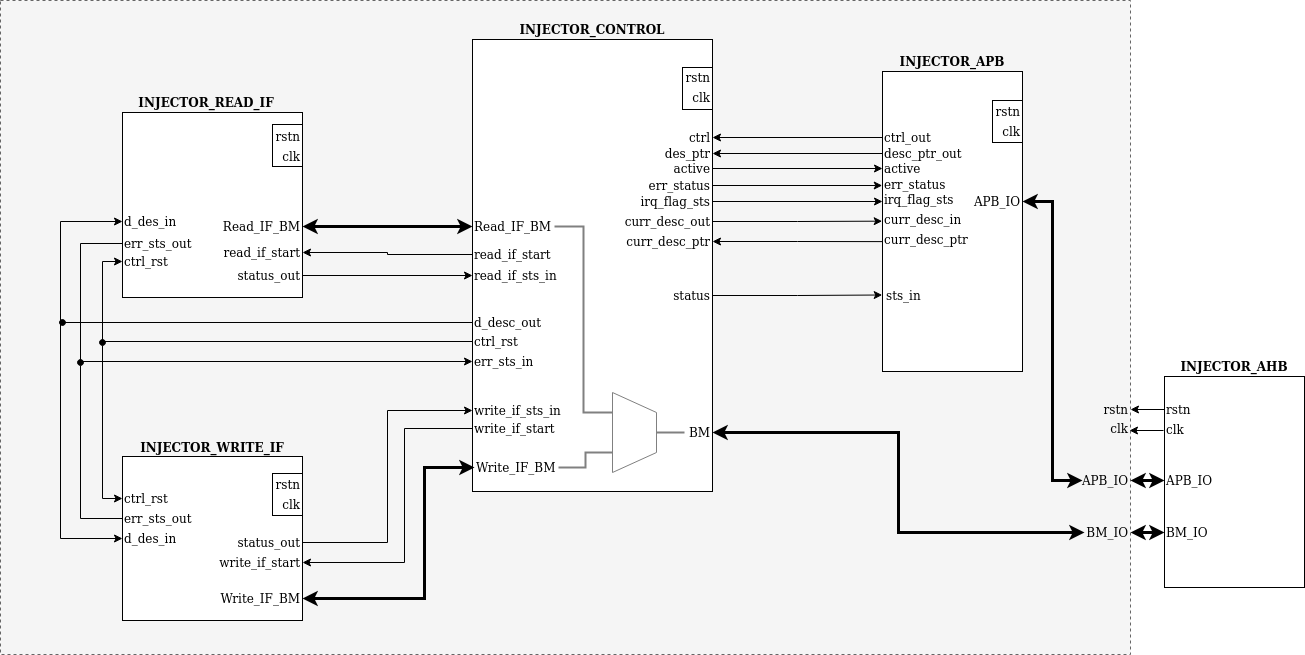
\includegraphics[width=15cm]{img/injector_low_level.pdf}
  \caption{Module internal block diagram and entity ports}
  \label{figure:low_level}
\end{figure}




\subsection{Subsystem modules}
\label{submodules}

\subsubsection{AHB Master Interface}
The injector has an AHB master port interfacing between the system bus and the control unit signals.\\
Bus master interface front end data width can be configured to 32, 64, or 128 bits based on the VHDL generic \code{dbits}. 
Burst accesses are always limited by a 1KB boundary as specified in AMBA 2.0. Moreover, in De-RISC and SELENE, the Bus is configured for up to 512B bursts. 
When a burst finishes, or if the descriptor is set up above the permitted burst limit, the burst will be interrupted at the specified memory boundary. An idle cycle will be inserted making re-arbitration on the AHB bus more frequent.

\subsubsection{APB Slave Interface}\label{section:apb}

\paragraph{Register specifications}
The traffic injector is controlled and monitored through registers mapped into a defined APB address space using the VHDL generics \code{paddr} and \code{pmask} as described in Table \ref{table:generics}.\\
The current injector version implements the shown registers in Table \ref{table:apb_registers}. Note how descriptors ranging from \code{0x10} up to \code{0x24} are used for debug capabilities and could be disabled to reduce the module footprint without losing any feature.

\begin{table}[ht]
	\scriptsize
	\centering
	\begin{tabular}{ll}
		\hline
		APB Address Offset & Register
		\\
		\hline
		0x00 & Control Register
		\\
		0x04 & Status Register
		\\
		0x08 & First descriptor pointer
		\\
		0x0C & Future capabilities register
		\\
		0x10 & \textbf{Debug} Descriptor control word
		\\
		0x14 & \textbf{Debug} Next descriptor pointer
		\\
		0x18 & \textbf{Debug} Destination address
		\\
		0x1C & \textbf{Debug} Source address
		\\
		0x20 & \textbf{Debug} Descriptor status
		\\
		0x24 & \textbf{Debug} Current descriptor pointer
		\\
		\hline
	\end{tabular}
	\caption{APB register map}
	\label{table:apb_registers}
\end{table}

% CONTROL REGISTER
\newpage
\paragraph{Control} %need subparagraph
The Control register allows the configuration of interrupt generation on error and descriptor completion. There are designated bits which allows different functionalities like kicking, enabling, resetting and enabling the QMode.\\
\begin{register}{H}{Control register}{CTRL~-~0x00}
    \label{reg_control}%
    \regfield{Reserved}{26}{6}{0}%
    \regfield{QM}{1}{5}{0}%
    \regfield{IER}{1}{4}{0}%
    \regfield{IE}{1}{3}{0}%
    \regfield{KCK}{1}{2}{0}%
    \regfield{RST}{1}{1}{0}%
    \regfield{EN}{1}{0}{0}%
    \reglabel{Reset}\regnewline%
    \begin{regdesc}\begin{reglist}[Request~Depth]
        \item [QM]Queue mode:
		\begin{itemize}
  		\item 0: Sequential queue
  		\item 1: Circular queue
		\end{itemize}
        \item [IER]Enable interrupt on error events.
        \item [IE]\begin{itemize}
  		\item 0: Disable interrupt
  		\item 1: Enable interrupt
		\end{itemize}
        \item [KCK]Kick Injector. Reads the current descriptor next address again 
	(if an error occurs or new descriptor is added to the completed queue).
        \item [RST]Reset injector. Setting this bit to one resets the core completely.
        \item [EN]Enable Injector controller
		\begin{itemize}
  		\item 0: Disabled
  		\item 1: Enabled
		\end{itemize}
\end{reglist}\end{regdesc}\end{register}


% STATUS REGISTER
\newpage
\paragraph{Status}
Display of any error specified in \ref{section:descriptors}, current injector status from its internal FSM, and completion monitoring.\\
\vspace{0.3cm}

\begin{register}{H}{Status register}{STS~-~0x04}
    \label{reg_sts}
    \regfield{Reserved}{11}{21}{0}%
    \regfield{CNT}{6}{15}{0}%
    \regfield{ST}{5}{10}{0}%
    \regfield{NPE}{1}{9}{0}%
    \regfield{WDE}{1}{8}{0}%
    \regfield{RDE}{1}{7}{0}%
    \regfield{RE}{1}{6}{0}%
    \regfield{DE}{1}{5}{0}%
    \regfield{IF}{1}{4}{0}%
    \regfield{KCK}{1}{3}{0}%
    \regfield{ONG}{1}{2}{0}%
    \regfield{ERR}{1}{1}{0}%
    \regfield{CMP}{1}{0}{0}%
    \reglabel{Reset}\regnewline%
    \begin{regdesc}\begin{reglist}[Request~Depth]
        \item [CNT]Current transaction repetition count value.
        \item [ST]Current Injector operation state.
        \item [NPE]Error while reading next descriptor pointer register.
        \item [WDE]Error while witing data during Control to Master transaction. Write Interface error.
        \item [RDE]Error while reading data during Master to Control transaction. Read Interface error.
        \item [RE]Read descriptor error.
        \item [DE]Decode descriptor error.
        \item [IF]Interrupt flag.
        \item [KCK]Kick flag pending to be executed.
        \item [ONG]Ongoing descriptor queue execution.
        \item [ERR]Error flag during descriptor queue execution.
        \item [CMP]Completed execution of the descriptor queue.
\end{reglist}\end{regdesc}\end{register}


%FIRST DESCRIPTOR POINTER
\paragraph{First descriptor pointer} Defines the first address where the first descriptor is allocated.\\

\begin{register}{H}{First descriptor pointer}{FPTR~-~0x08}
    \label{reg_fptr}%
    \regfield{addr}{32}{0}{0}%
    \reglabel{Reset}\regnewline%
    \begin{regdesc}\begin{reglist}[Request~Depth]
        \item [addr]First descriptor pointer register. Points to the first descriptor of the queue.
\end{reglist}\end{regdesc}\end{register}


% FUTURE CAPABILITIES REGISTER
\newpage
\paragraph{Future capabilities} It is a reserved register that has already been specified for future module releases. Just like the \textbf{Debug APB Registers}, this register can be disabled.\\

\begin{register}{H}{Future capabilities register}{FCPB~-~0x0C}
    \label{reg_fcpb}%
    \regfield{Reserved}{32}{0}{0}%
    \reglabel{Reset}\regnewline%
    \begin{regdesc}\begin{reglist}[Request~Depth]
        \item [Reserved] This register is reserved for future features.
\end{reglist}\end{regdesc}\end{register}


%DEBUG: DESCRIPTOR CONTROL WORD
\paragraph{Descriptor control word for debug capability}.\\

\begin{register}{H}{Descriptor control word for debug capability}{DCTR~-~0x010}
    \label{reg_dctr}%
    \regfield{ctrl}{32}{0}{0}%
    \reglabel{Reset}\regnewline%
    \begin{regdesc}\begin{reglist}[Request~Depth]
        \item [ctrl]Current descriptor's control field for debug capability.
\end{reglist}\end{regdesc}\end{register}


% DEBUG: NEXT DESCRIPTOR POINTER
\paragraph{Next descriptor pointer for debug capability}.\\

\begin{register}{H}{Next descriptor pointer for debug capability}{DNXT~-~0x014}
    \label{reg_dnxt}%
    \regfield{addr}{32}{0}{0}%
    \reglabel{Reset}\regnewline%
    \begin{regdesc}\begin{reglist}[Request~Depth]
        \item [addr]Next descriptor field for debug capability.
\end{reglist}\end{regdesc}\end{register}

\newpage
% DEBUG: DESTINATION ADDRESS
\paragraph{Destination address for debug capability}.\\

\begin{register}{H}{Destination address for debug capability}{DDST~-~0x018}
    \label{reg_ddst}%
    \regfield{addr}{32}{0}{0}%
    \reglabel{Reset}\regnewline%
    \begin{regdesc}\begin{reglist}[Request~Depth]
        \item [addr]Current descriptor’s destination address field for debug capability.
\end{reglist}\end{regdesc}\end{register}


% DEBUG: SOURCE ADDRESS
\paragraph{Source address for debug capability}.\\

\begin{register}{H}{Source address for debug capability}{DSRC~-~0x01C}
    \label{reg_dsrc}%
    \regfield{addr}{32}{0}{0}%
    \reglabel{Reset}\regnewline%
    \begin{regdesc}\begin{reglist}[Request~Depth]
        \item [addr]Current descriptor’s source address field for debug capability.
\end{reglist}\end{regdesc}\end{register}


% DEBUG: DESCRIPTOR STATUS
\paragraph{Descriptor descriptor status for debug capability}.\\

\begin{register}{H}{Descriptor status for debug capability}{DSTS~-~0x020}
    \label{reg_dsts}%
    \regfield{sts}{32}{0}{0}%
    \reglabel{Reset}\regnewline%
    \begin{regdesc}\begin{reglist}[Request~Depth]
        \item [sts]Current descriptor’s status word for debug capability.
\end{reglist}\end{regdesc}\end{register}


% DEBUG: CURRENT DESCRIPTOR POINTER
\paragraph{Current descriptor pointer for debug capability}.\\

\begin{register}{H}{Current descriptor pointer debug capability}{DPTR~-~0x024}
    \label{reg_dptr}%
    \regfield{addr}{32}{0}{0}%
    \reglabel{Reset}\regnewline%
    \begin{regdesc}\begin{reglist}[Request~Depth]
        \item [addr]Pointer from which the current descriptor is read, for debug capability.
\end{reglist}\end{regdesc}\end{register}





\newpage
\subsubsection{Control Unit}
The control unit is in charge of decoding descriptors and routes the transaction requests to the respective sub-modules (either take control of the \textbf{Read Interface}, \textbf{Write Interface} or \textbf{Delay Interface}). Also, it is used to monitor the status and errors of these transactions and report them back to the APB Interface. 
A finite state machine is implemented in order to achieve this functionality.\\
\begin{figure}[ht]
	\centering
	\begin{tikzpicture}
		\node[state, accepting] (1) {$1$};
		\node[state, below right of=1, xshift=1cm] (2) {$2$};
		\node[state, right of=2] (3) {$3$};
		\node[state, below of=2, yshift=-1cm] (4) {$4$};
		\node[state, below of=1] (5) {$5$};
		\node[state, below of=5] (6) {$6$};
	
		\draw	(1) edge[loop above] node{$err$} (1)
				(1) edge[right, bend left, right=0.3] node{$next\_desc$} (2)
				(2) edge[loop right] node{$wait$} (2)
				(2) edge[below, bend left, above=0.3] node{$req\_grant$} (3)
				(3) edge[right, bend right, right=0.3] node{$err$} (1)
				(3) edge[below, bend left, right=0.3] node{$ok$} (4)
				(4) edge[above, bend right, above=0.3] node{$read\_type$} (5)
				(4) edge[left, bend right, left=0.3] node{$err$} (1)
				(4) edge[below, bend left, right=0.3] node{$write\_type$} (6)
				(5) edge[left, left=0.3] node{$q\_mode$} (4)
				(5) edge[left, bend left, left=0.3] node{$ok$} (1)
				(6) edge[left, above=0.3] node{$q\_mode$} (4)
				(6) edge[left, bend left, left=0.3] node{$ok$} (1);
	\end{tikzpicture}
	\caption{Control unit FSM diagram}
	\label{fig:control_states}
\end{figure}

\paragraph{Description}
\subparagraph{1. Idle}
Execution starts from Idle state and comes back after completion of each descriptor write to FIFO and on FIFO completion. The core processes a descriptor only if no errors have been encountered and if the core is enabled. If the execution is ongoing and is not the last descriptor, the core proceeds with the next descriptor fetch. Else if the whole queue is completed, execution is paused, and the core stays idle. If the core is disabled or an error occurred, the Injector goes into a disabled state and shows the corresponding error flag.

\subparagraph{2. Fetch Descriptor}
Initiates a 20 Byte long burst read through the Bus Master Interface to read the descriptor fields.

\subparagraph{3. Read Descriptor}
Once they are read, we save the descriptor fields to the corresponding FIFO position to be executed later on.

\subparagraph{4. Read FIFO}
When all descriptors are loaded into the FIFO or the FIFO is full, the first position is read and stored in internal descriptor registers for decoding. Once all the descriptors are executed, execution goes back to Idle state and marks the completion flags.

\subparagraph{5. Decode Descriptor}
Checks if the descriptor is enabled. Disabled descriptors are skipped and core jumps to read FIFO to proceed with the next descriptor in the queue.\\
If the descriptor is enabled, based on the \code{desc\_type} field value, it decodes the type of the descriptor and jumps to respective states:
\begin{itemize}
 	\item \textbf{Read descriptor type}: It sends \code{read\_if\_start} signal to the \code{injector\_read\_if} sub-module.
  	\item \textbf{Write descriptor type}: It sends a \code{write\_if\_start} signal to the \code{injector\_write\_if} sub-module.
	\item \textbf{Delay descriptor type}: It sends a \code{delay\_if\_start} signal to the \code{injector\_delay\_if} sub-module.
\end{itemize}

\subparagraph{6. Read I/F}
Always monitors for any errors and status from \code{injector\_read\_if} sub-module. If an error is reported from the read interface sub-module, it handles the error. When a \code{read\_if\_comp} status is received, the core checks for the \textbf{Repetition count value}, it jumps to state five and starts the same descriptor again. If not, the core jumps to read FIFO state and sends a completed signal..

\subparagraph{7. Write I/F}
Always monitors for any errors and status from \code{injector\_write\_if} module. If an error is reported from its interface sub-module, it handles the error. When a \code{write\_if\_comp} status is received, the core checks for the \textbf{Repetition count value}, it jumps to state five and starts the same descriptor again. If not, the core jumps to read FIFO state and sends a completed signal.\\

\subparagraph{7. Delay I/F}
Always monitors for any errors and status from \code{injector\_delay\_if} module. If an error is reported from its interface sub-module, it handles the error. When a \code{delay\_if\_comp} status is received, the core checks for the \textbf{Repetition count value}, it jumps to state five and starts the same descriptor again. If not, the core jumps to read FIFO state and sends a completed signal.\\
\vspace{1cm}





\newpage
\subsubsection{Read Interface Module}
The Injector Read Interface deals with data fetch from memory. The descriptor fields are passed from the injector control sub-module.\\
The Read Interface will continue executing until the transaction size specified in the current descriptor size field is completely transferred.\\

\begin{figure}[ht]
	\centering
	\begin{tikzpicture}
		\node[state, accepting] (1) {$1$};
		\node[state, right of=1,xshift=1cm] (2) {$2$};
		\node[state, below left of=2,yshift=-2cm] (3) {$3$};
	
		\draw	(1) edge[right,below=0.3] node{$read\_start$} (2)
				(1) edge[loop above] node{$wait$} (1)
				(2) edge[left,bend right, above=0.3] node{$comp$} (1)
				(2) edge[below,bend left,right=0.3] node{$req\_grant$} (3)
				(3) edge[left] node{$buf\_full$} (2)
				(3) edge[left, bend left, left=0.3] node{$remaining=0$} (1)
				(3) edge[left, pos=.3, left=0.3] node{$err$} (1);
	\end{tikzpicture}
	\caption{Read Interface FSM diagram}
	\label{fig:read_states}
\end{figure}

\paragraph{Description}
\subparagraph{1. Idle}
Its the starting state. Waits for \code{read\_start\_in} signal to proceed. Decides what size of the current burst is to be transferred depending on the descriptor parameters.

\subparagraph{2. Execute Data Descriptor}
Initiates a bus master interface burst read transfer with the specified source address and transaction size.

\subparagraph{3. Read Data}
Reads each data word from the bus master interface output until the total data is transferred.\\
\vspace{1cm}
\newpage
\subsubsection{Write interface module}
The Write Interface module deals with data write transactions to AHB Addresses.\\
Data descriptor fields are passed from the control sub-module, and \code{write\_if\_start} signal is asserted only for enabled descriptors.
Once the dummy data (a 32-bit array of 1's) is completely transferred to memory according to the specified size in the descriptor control word field, execution stops the Write Interface operation. It goes back to the main control state machine in the injector control.\\

\begin{figure}[ht]
	\centering
	\begin{tikzpicture}
		\node[state, accepting] (1) {$1$};
		\node[state, below of=1] (2) {$2$};
		\node[state, below right of=2] (3) {$3$};
		\node[state, below left of=2] (4) {$4$};
		\draw	(1) edge[right,bend left,right=0.3] node{$write\_if\_start$} (2)
				(1) edge[loop above] node{$wait$} (1)
				(2) edge[left,bend left, left=0.3] node{$size=0$} (1)
				(2) edge[below,bend left,right=0.3] node{$size>0$} (3)
				(2) edge[below,bend left,right=0.3] node{$size\_left=0$} (4)
				(3) edge[loop right] node{$more\_data$} (3)
				(3) edge[left, bend left, below=0.3] node{$size=0$} (4)
				(4) edge[left,bend left,below=0.3] node{$size\_left!=0$} (2)
				(4) edge[left,bend left,pos=.3, left=0.3] node{$comp$} (1);
	\end{tikzpicture}
	\caption{Write Interface FSM diagram}
	\label{fig:write_states}
\end{figure}

\paragraph{Description}
\subparagraph{1. Idle}
Starting state, waits for \code{write\_if\_start} signal from the control sub-module to proceed.

\subparagraph{2. First Word}
If there is data to be written, the FSM proceeds to fetch and compute the transfer's addresses and sizes and starts a normal 4 byte aligned or burst transfer.

\subparagraph{3. Write Burst}
If we still have data after a first 4-byte transfer, a burst transaction starts and loops until finished.

\subparagraph{4. Write  Data Check}
Once a normal transaction or burst transaction ends, we check if we need to start another burst (we have to keep in mind the upper bound on the permitted burst size) or the transaction has finished.\\[0.5cm]



\newpage
\subsubsection{Delay Interface Module}
The Injector Delay Interface transaction delays between executions. The descriptor fields are passed from the injector control sub-module.\\
The Delay Interface will continue executing until the transaction size (delay size) specified in the descriptor size field is completed.\\

\begin{figure}[ht]
	\centering
	\begin{tikzpicture}
		\node[state, accepting] (1) {$1$};
		\node[state, right of=1,xshift=1cm] (2) {$2$};
	
		\draw	(1) edge[right,below=0.3] node{$delay\_start$} (2)
				(1) edge[loop above] node{$wait$} (1)
				(2) edge[left,bend right, above=0.3] node{$comp$} (1);
	\end{tikzpicture}
	\caption{Delay Interface FSM diagram}
	\label{fig:read_states}
\end{figure}

\paragraph{Description}
\subparagraph{1. Idle}
Its the starting state. Waits for \code{delay\_start\_in} signal to proceed. Decides what size of the current delay is to be executed depending on the descriptor parameters.

\subparagraph{2. Execute Descriptor}
Initiates a clock counter countdown with the specified size. Returns to Idle when finished.

\vspace{1cm}










\end{document}
